\documentclass[11pt,a4paper]{scrartcl}
\typearea{12}
\usepackage{graphicx}
\usepackage{pstricks}
\usepackage{listings}


\usepackage{graphicx}

\usepackage{tikz}
\usetikzlibrary{positioning}
\usetikzlibrary{arrows,automata}
\usetikzlibrary{decorations.markings}
\usetikzlibrary{calc}

\lstset{language=python}
\pagestyle{headings}
\markright{Computation Neuroscience - 6 synapses}
\begin{document}

\subsection*{Chemical synapses}

Spikes, the voltage pulses that carry signals from neuron to neuron,
are notably stereotypical; there aren't big spikes and small spikes,
to a good approximation, there are just spikes. However, the effect
one neuron has on the other can vary considerably, not just from
neuron to neuron, but from time to time. This variablity can occur
because of chemical synapses, the complicated biochemical machinery
responsible for connect the axon of one neuron to the dendrite of
another. 

Chemical synapses are not the only synapses, there are also
\textsl{gap junction}. If an axon is connected to a dendrite by a gap
junction there is a small hole directly connecting the inside of one
neuron through to the inside of the other, usually this means that the
axon of one neuron is connected to the dentrite of the other, though
axon to axon gap junctions are also found. For an axon to dentrite gap
junction this means that when a spike travelling along the axon
reaches the gap junction some of the charged ions diffuse through the
gap changing the charge in the dendrite. In some simple animals like
jelly fish most or all of the synapses are gap junctions. There are
gap junctions in the mammalian brain, for example gap junctions are
thought to be responsible for the dynamics which supports very rapid
oscillations in the hippocampus, however, most of the synapses in the
mammalian brain are chemical synapses. We will see that this allows a
more variable effect of a pre-synaptic spike on the voltage of the
post-synaptic dendrite.

In a chemical synapse the pre-synaptic spike does not effect the
post-synaptic voltage directly, instead it causes a cascade of
bio-electrodynamics events which ultimately causes a transient change
in conductance of the post-synaptic membrane. 

Roughly, the synapse consists of a protuberance in the axon called the
\textsl{terminal bouton}, the terminal bouton is held by astocyte,
supporting non-neuronal brain cells, so that it is separated by a tiny
gap, called the \textsl{synaptic cleft} from a bump in the dendrite
called the \textsl{dendritic spine}. The terminal bouton is filled
with tiny bags or bubbles called \textsl{vesicles}, these contain
special molecules called \textsl{neurotransmitters}. When a spike
arrives at the terminal bouton it causes calcium gates to open in the
cellular membrane, the resulting influx of calcium ions causes some of
the vesicles to migrate to the membrane separating the bouton from the
synaptic cleft, they burst releasing neurotransmitter into the cleft. 

\begin{figure}
\begin{center}
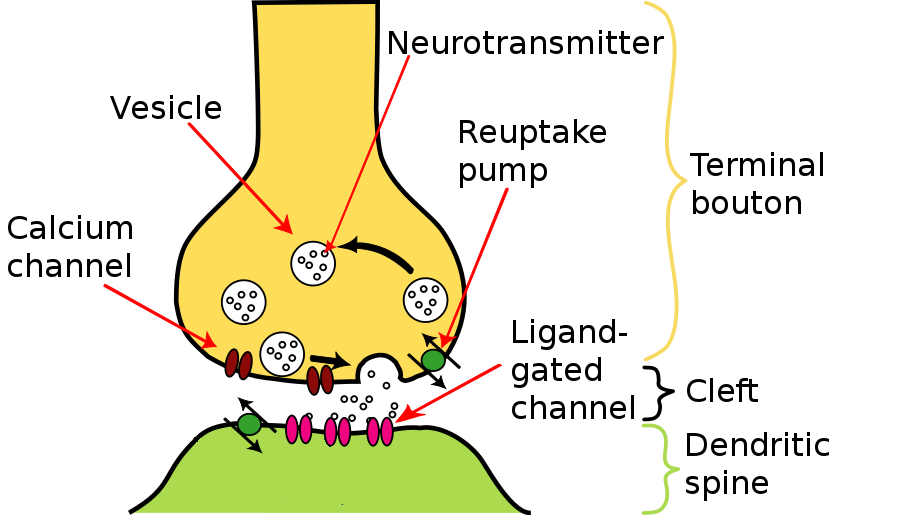
\includegraphics[width=12cm]{Synapse.png}
\end{center}
\caption{The major parts of the synapse; this shows a vesicle
  bursting, releasing neurotransmitter into the cleft, this will bind
  with the ligand-gated channels to allow a current across the
  membrane of the dendrite. Reuptake pumps are shown in the bouton and
  the spine, there are also pumps in the astrocyte that surrounds the
  cleft but isn't shown here. Some is also lost to diffusion. [Diagram
    modified from one in wikipedia.]}
\end{figure}


The membrane of the dendritic is pieced by gated ion channels; these
are \textsl{ligand gated} channels. This means that they contain a
receptor site which binds with a particular type of molecule, like a
key designed for the receptor site's lock. When the receptor has a
molecule bound to it, the gate is open and so ions can pass through
the channel, like the other channels we have seen the channel is ion
specific, so only one type of ion can pass through it. In the case of
the ligand-gated channels in the dendritic spine, the neurotransmitter
binds with the receptor, opening the gate. Hence, after a spike
arrives at the synapse the cleft is filled with neurotransmitter and
some of that neurotransmitter binds to the gated channels, causing
them to open. This in turn allows a flow of ions in or out of the
dendrite, changing the voltage there. A cartoon of a ligand-gated
channel is given in Fig.~\ref{LGIC}.

\begin{figure}
\begin{center}
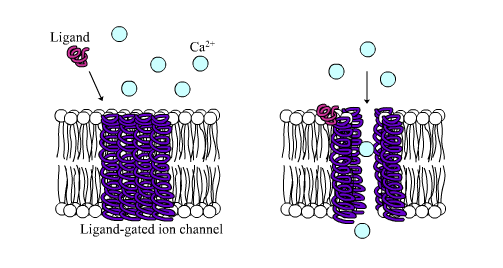
\includegraphics[width=12cm]{LGIC.png}
\end{center}
\caption{Sketch of a ligand-gated channel; when the neurotransmitter,
  the ligand, binds to the gate it opens allowing the ions to pass
  through. This is a Calcium channel, calcium, like sodium, is found
  in higher concentrations outside the cell so the chemical gradient,
  as well as the voltage gradient, means these ions flow into the cell
  from outside, increasing its potential.  This is therefore part of
  an excitatory synapse. Inhibitory synapses have ligand-gated
  potassium and chlorine channels, potassium, as we have discussed, is
  at a higher concentration inside the cell and so will flow out,
  depending on the voltage gradient, lowering the potential inside the
  cell. Chlorine is at a higher concentration outside the cell but is
  a negative ion, so when it flows in it also lowers the
  potential.[Diagram modified from wikipedia.]\label{LGIC}}
\end{figure}


Which ion and which direction, depends on the synapses, we will return
to that. For now, though, let us continue describing what happen;
after the neurotransmitter floods the cleft it is quickly reabsorbed
though neurotransmitter reuptake pumps. Some of the neurotransmitter
is absorbed into the bouton, some into the spine and some is absorbed
by the astrocyte, the important thing is that the concentration of
neurotransmitter in the cleft falls rapidly. Now, the fluid of the
cleft has little neurotransmitter, but there is still neurotransmitter
bound to the receptors of the ligand gated channels. This gradually
unbinds, this is usually imagined to be a random process, because of
the Brownian motion of molecules in the fluid of the cleft and the
thermal vibration of the receptor itself, the neurotransmitters unbind
as the result of random collisions and thermal variations. As they do
so, the channels close again and the conductivity of the dendritic
spine's membrane falls back towards zero.

\subsection*{Post-synaptic potential}

One important property of neurons is that a given neuron is either
\textsl{excitatory} or \textsl{inhibitory}. If a neuron is excitatory,
this means all its synapses are excitatory, that is, they make the
post-synaptic neuron more likely to spike by increasing its
voltage. In an excitatory neuron opening the ligand-gated channels
causes a positive current into the cell, typically this means that
they are sodium or calcium channels, so that when they open positive
sodium or calcium ions flow into the dendrite. Conversely, if a neuron
is inhibitory all its synapses are inhibitory, they make the
post-synaptic cell less likely to fire by decreasing its voltage. In
an inhibitory synapse opening the ligand-gated channels causes a
positive flow out of the dendrite, lowering the voltage. Typically
inhibitory channels are either potassium gates, allowing postive
potassium to leave the dendrite, or chlorine gates, allowing
negatively charged chlorine to flow in.

The post-synaptic change in potential that results from a pre-synaptic
spike is called a \textsl{post-synaptic potential}; if the synapse is
excitatory this is called an \textsl{excitatory post-synaptic
  potential} or EPSP, if it is inhibitory it is called an
\textsl{inhibitory post-synaptic potential} or IPSP. The profile of
PSPs reflects the neurotransmitter dynamics, it rises fast as the
neurotransmitter floods the cleft and the ion-channels open, it then
decays back to zero following an exponential decay, reflecting the
constant rate unbinding process: since any bound molecule has a
constant probability of shaking free the number of unbinding events
depends on the number of bound molecules, giving an exponential decay.

Often the post-synaptic condutivity is taken to be a what is called an
$alpha$ function:
\begin{equation}
I_s(t)=g_ss(t)(V-E_s)
\end{equation}
where $I_s(t)$ is the synpatic current, $E_s$ is the reversal
potential of the synapse and $g_ss(t)$ is the conductance, $g_s$ is a
constant describing the strength of the synapse and $s(t)$ is 
\begin{equation}
s(t)=te^{-t/\tau_s}
\end{equation}
where $\tau_s$ is a time scale, see Fig.~\ref{fig:alpha}. Basically
the rising part of the $\alpha$ function models the period when there
is neurotransmitter in the cleft, this is binding to the channels
increasing the conductance; the falling part represents the period
where the unbound neurotransmitter has been cleared from the cleft and
the bound neurotransmitter is unbinding randomly due to the thermal
motion of molecules. It is possible to understand these dynamics in
terms of the bucket-like equations we have examined before, but this
won't be done here.

\begin{figure}
\begin{center}
% GNUPLOT: LaTeX picture with Postscript
\begingroup
  \makeatletter
  \providecommand\color[2][]{%
    \GenericError{(gnuplot) \space\space\space\@spaces}{%
      Package color not loaded in conjunction with
      terminal option `colourtext'%
    }{See the gnuplot documentation for explanation.%
    }{Either use 'blacktext' in gnuplot or load the package
      color.sty in LaTeX.}%
    \renewcommand\color[2][]{}%
  }%
  \providecommand\includegraphics[2][]{%
    \GenericError{(gnuplot) \space\space\space\@spaces}{%
      Package graphicx or graphics not loaded%
    }{See the gnuplot documentation for explanation.%
    }{The gnuplot epslatex terminal needs graphicx.sty or graphics.sty.}%
    \renewcommand\includegraphics[2][]{}%
  }%
  \providecommand\rotatebox[2]{#2}%
  \@ifundefined{ifGPcolor}{%
    \newif\ifGPcolor
    \GPcolorfalse
  }{}%
  \@ifundefined{ifGPblacktext}{%
    \newif\ifGPblacktext
    \GPblacktexttrue
  }{}%
  % define a \g@addto@macro without @ in the name:
  \let\gplgaddtomacro\g@addto@macro
  % define empty templates for all commands taking text:
  \gdef\gplbacktext{}%
  \gdef\gplfronttext{}%
  \makeatother
  \ifGPblacktext
    % no textcolor at all
    \def\colorrgb#1{}%
    \def\colorgray#1{}%
  \else
    % gray or color?
    \ifGPcolor
      \def\colorrgb#1{\color[rgb]{#1}}%
      \def\colorgray#1{\color[gray]{#1}}%
      \expandafter\def\csname LTw\endcsname{\color{white}}%
      \expandafter\def\csname LTb\endcsname{\color{black}}%
      \expandafter\def\csname LTa\endcsname{\color{black}}%
      \expandafter\def\csname LT0\endcsname{\color[rgb]{1,0,0}}%
      \expandafter\def\csname LT1\endcsname{\color[rgb]{0,1,0}}%
      \expandafter\def\csname LT2\endcsname{\color[rgb]{0,0,1}}%
      \expandafter\def\csname LT3\endcsname{\color[rgb]{1,0,1}}%
      \expandafter\def\csname LT4\endcsname{\color[rgb]{0,1,1}}%
      \expandafter\def\csname LT5\endcsname{\color[rgb]{1,1,0}}%
      \expandafter\def\csname LT6\endcsname{\color[rgb]{0,0,0}}%
      \expandafter\def\csname LT7\endcsname{\color[rgb]{1,0.3,0}}%
      \expandafter\def\csname LT8\endcsname{\color[rgb]{0.5,0.5,0.5}}%
    \else
      % gray
      \def\colorrgb#1{\color{black}}%
      \def\colorgray#1{\color[gray]{#1}}%
      \expandafter\def\csname LTw\endcsname{\color{white}}%
      \expandafter\def\csname LTb\endcsname{\color{black}}%
      \expandafter\def\csname LTa\endcsname{\color{black}}%
      \expandafter\def\csname LT0\endcsname{\color{black}}%
      \expandafter\def\csname LT1\endcsname{\color{black}}%
      \expandafter\def\csname LT2\endcsname{\color{black}}%
      \expandafter\def\csname LT3\endcsname{\color{black}}%
      \expandafter\def\csname LT4\endcsname{\color{black}}%
      \expandafter\def\csname LT5\endcsname{\color{black}}%
      \expandafter\def\csname LT6\endcsname{\color{black}}%
      \expandafter\def\csname LT7\endcsname{\color{black}}%
      \expandafter\def\csname LT8\endcsname{\color{black}}%
    \fi
  \fi
  \setlength{\unitlength}{0.0500bp}%
  \begin{picture}(5040.00,3528.00)%
    \gplgaddtomacro\gplbacktext{%
      \csname LTb\endcsname%
      \put(1210,704){\makebox(0,0)[r]{\strut{} 0}}%
      \put(1210,1344){\makebox(0,0)[r]{\strut{} 0.001}}%
      \put(1210,1983){\makebox(0,0)[r]{\strut{} 0.002}}%
      \put(1210,2623){\makebox(0,0)[r]{\strut{} 0.003}}%
      \put(1210,3262){\makebox(0,0)[r]{\strut{} 0.004}}%
      \put(1342,484){\makebox(0,0){\strut{} 0}}%
      \put(2002,484){\makebox(0,0){\strut{} 0.02}}%
      \put(2662,484){\makebox(0,0){\strut{} 0.04}}%
      \put(3323,484){\makebox(0,0){\strut{} 0.06}}%
      \put(3983,484){\makebox(0,0){\strut{} 0.08}}%
      \put(4643,484){\makebox(0,0){\strut{} 0.1}}%
      \put(176,1983){\rotatebox{-270}{\makebox(0,0){\strut{}$s(t)$}}}%
      \put(2992,154){\makebox(0,0){\strut{}$t$}}%
    }%
    \gplgaddtomacro\gplfronttext{%
      \csname LTb\endcsname%
      \put(3656,3090){\makebox(0,0)[r]{\strut{}$t\exp{(-t/0.01)}$}}%
    }%
    \gplbacktext
    \put(0,0){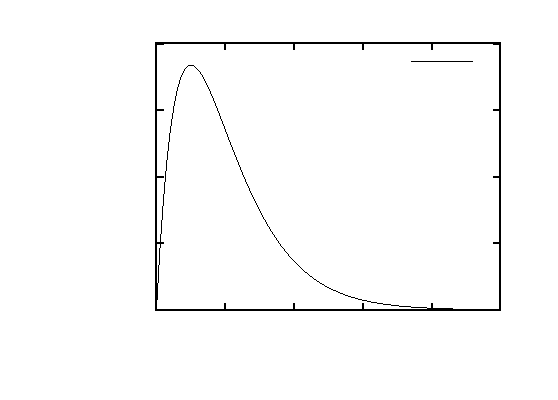
\includegraphics{alpha}}%
    \gplfronttext
  \end{picture}%
\endgroup

\end{center}
\caption{The $\alpha$-function profile often used to model synaptic
  conductances, shown here with $\tau_m=10$ ms.\label{fig:alpha}}
\end{figure}

\subsection*{The complexity of synapses}

The chemical synapse is complicated and there are many details of the
synapse that can effect the dynamics. For example, the strength of the
synapse, that is, the amplitude of the change in conductance that
follows a pre-synaptic spike, depends on the number of vesicles
released, on the size of the cleft, the speed of reuptake and the
number of ligand-gated channels; the shape and duration of the PSP
depends on the detailed dynamics of binding, reuptake and unbinding
and the effect of the PSP on the post-synaptic soma depends on the
shape of the dendritic tree and the details of the diffusive process
which conducts the PSP to the soma, a distal synapse will have a
different effect to a proximal one. The shape of the dendritic spine
can also filter the PSP, modulating its shape.

Some aspects of synaptic dynamics vary from synapse to synapse;
usually the length of a timescale depends on the neurotransmitter and
receptor; excitatory synapses tend to have shorter time constants than
inhibitory ones, but excitatory synapses have two common receptors for
glutamate, the most common excitatory transmitter: NMDA-receptors
which are quick and AMPA receptors, which are slow. In the case of
inhibitory synapses the most common transmitter is called GABA and the
common receptors are the simpler GABA-A receptor and the more
complicated GABA-B receptors. We will see that some special synapses
release neuromodulators rather than neurotransmitters; these often
change behaviors in subtler ways.

There are typically spike-to-spike effects usually described as
\textsl{short term plasticity}, for example if two spikes arrive one
soon after the other, the first might have already opened a
substantial quantity of the gates, reducing the effect of the second.
If there is a high rate of pre-synaptic spike arrivals the vesicles
may be depleted reducing the size of PSPs, this is called
\textsl{short term depression}; sometimes the opposite is true, the
build up of calcium ions in response to a high rate of pre-synaptic
spiking can increase the size of PSPs, this is \textsl{short term
  facilitation}. Short term plastic effects, with timescales of 10 ms
up to seconds are thought to play an important role in neural
computation \cite{AbbottEtAll1997a}. This short term plasticity is
usually distinguished from long term plasticity, the long term changes
in the structure of the synapses that are thought to be responsible
for learning and development in the brain.

\subsection*{Synaptic plasticity}

Synaptic plasticity usually refers to the long-term changes in synapse
strength, an long term increase in synaptic strength is called
\textsl{long term potentiation} of LTP, a decrease is called
\textsl{long term depression} or LTD. It is believed that synapses
respond to their pre- and post-synaptic activity, so that the changes
depend on the behavior of the pre- and post-synaptic neurons. It is
not known in detail what rules govern this plasticity, it seems
different neurons have different plasticity rules. 

The closest thing to an overall rule was formulated by Hebb in 1949
when he said \cite{Hebb1949a}:
\begin{quote}
Let us assume that the persistence or repetition of a reverberatory
activity (or \lq{}trace\rq{}) tends to induce lasting cellular changes that
add to its stability. [$\ldots$] When an axon of cell A is near enough to excite
a cell B and repeatedly or persistently takes part in firing it, some
growth process or metabolic change takes place in one or both cells
such that A's efficiency, as one of the cells firing B, is increased.
\end{quote}
In other words, if one neurons tends to cause another to fire, the
synapse from the first to the second will get stronger. In artificial
neural networks the nodes, modelling neurons, often lack spiking
dynamics and so have a continuous state or rate variable; since
\textsl{Hebbian plasticity} often plays a role in artificial neural
networks it is often applied to a rule that strengthens synapses
between neurons that are active at the same time, that is, the
explicit causal structure is ignored in favor of
\begin{quote}
Neurons that fire together wire together.
\end{quote}
This leads to a plasticity rule 
\begin{equation}
\delta w_{ij}=\eta x_i x_j
\end{equation}
where $w_{ij}$ is the strength of the synapse from neuron $i$ to
neuron $j$, $x_i$ and $x_j$ are the states of the two neurons and
$\eta$ is a learning rate. Another version isK or
\begin{equation}
\delta w_{ij}=\eta (x_i-\theta)(x_j-\theta)
\end{equation}
where $\theta$ is a threshold, this allows negative changes, when
$x_i>\theta$ and $x_j<\theta$, or visa versa.

\subsection*{Spike-timing dependent plasticity}

The late nineties saw a revival of interest in causal, spike-timing
based, plasticity rules. A series of papers pointed to experimental
evidence for timing effects in plasticity
\cite{MarkramSakmann1995a,MarkramEtAl1997a,BellEtAl1997a,MageeJohnston1997a,DebanneGahwilerThompson1998a}
including a definitive demonstration of a spike-order dependent
plastic changes \textsl{in vitro} in \cite{MarkramEtAl1997a}, the
observation of asymmetric STDP \textsl{in vivo} in developing Xenopus
in \cite{ZhangTaoHoltHarrisPoo1998a} and a clear graph of the time
dependence of plastic changes \textsl{in vitro} in \cite{BiPoo1998a}.

The famous graph of spike timing dependent plasticity is shown in
Fig.~\ref{fig:BiPoo}. This shows measurements of plastic changes made
in an \textsl{in vitro} preparation. Electrodes are inserted into two
synaptically connected cells and currents are used to cause both to
spike periodically with a gap of $\delta t$ between the pre- and
post-synaptic spikes. This causes the synaptic strength to change, if
the pre-synaptic spike precedes the post-synaptic spike the synapse
gets stronger with the degree of strengthening depending on the size
of $|\delta t|$, the bigger the gap the smaller the effect with a
roughly exponential profile. The opposite is observed if the
pre-synaptic spike arrives after the post-synaptic spike has left, in
this case the synapse gets weaker, again the size of the effect falls
like an exponential as $|\delta t|$ gets bigger.


\begin{figure}
\begin{center}
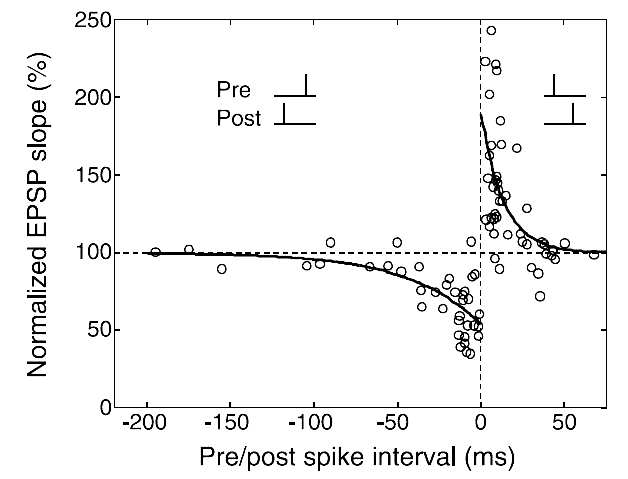
\includegraphics[width=12cm]{DanPoo2004.jpg}
\end{center}
\caption{Spike timing dependent plasticity. This shows the change in
  synapse strength as a function of the timing gap between the pre-
  and post-synaptic spike. \label{fig:BiPoo}}
\end{figure}

There are lots of caveats to be added to this, it is quite an
artificial situation, in vitro with periodic spiking; since the
changes are only tracked over a show period it isn't clear whether the
changes are additive
\begin{equation}
w\rightarrow w+\delta w
\end{equation}
or multiplicative
\begin{equation}
w\rightarrow \lambda_w w
\end{equation}
However, it does give a striking picture of how spike-timing dependant
plasticity (STDP) might work. 


\begin{figure}
\begin{center}
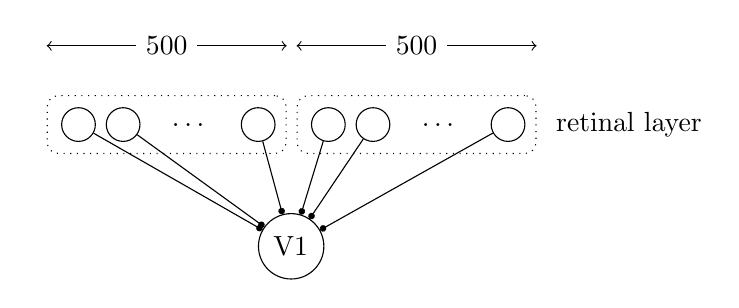
\begin{tikzpicture}
\node[rectangle,rounded corners,text width=2.8cm,text height=0.5cm,draw=black,dotted,align=left](a){};
\node[rectangle,rounded corners,text width=2.8cm,text height=0.5cm,draw=black,dotted,align=left, right = 0.125cm of a](b){};
\node[align=left, right = 0.125cm of b](text){retinal layer};
\node[left = 0cm of a](al){};
\node[right = 0cm of a](ar){};
\node[above of = al](aal){};
\node[above of = ar](aar){};
\node[above of = a](atext){500};
\path (atext) edge[->] (aal);
\path (atext) edge[->] (aar);
\node[left = 0cm of b](bl){};
\node[right = 0cm of b](br){};
\node[above of = bl](abl){};
\node[above of = br](abr){};
\node[above of = b](btext){500};
\path (btext) edge[->] (abl);
\path (btext) edge[->] (abr);

\node[right = -0.0675cm of a](ab){};

\node[circle,text width=0.125cm,draw=black,align=center,left = -0.625cm of a](a1){};
\node[circle,text width=0.125cm,draw=black,align=center,right = 0.125cm of a1](a2){};
\node[text width=0.125cm,align=center,right = 0.275cm of a2](adots){$\ldots$};
\node[circle,text width=0.125cm,draw=black,align=center,right = 0.625cm of adots](a3){};
\node[circle,text width=0.125cm,draw=black,align=center,left = -0.625cm of b](b1){};
\node[circle,text width=0.125cm,draw=black,align=center,right = 0.125cm of b1](b2){};
\node[text width=0.125cm,align=center,right = 0.275cm of b2](bdots){$\ldots$};
\node[circle,text width=0.125cm,draw=black,align=center,right = 0.625cm of bdots](b3){};

\node[circle,text width=0.45cm,draw=black,align = left,below = 1cm of ab](pc){V1};


\draw[
    decoration={markings,mark=at position 1 with {\arrow[scale = 0.5]{*}}},
    postaction={decorate}
    ]
    (a1) -- (pc);

\draw[
    decoration={markings,mark=at position 1 with {\arrow[scale = 0.5]{*}}},
    postaction={decorate}
    ]
    (a2) -- (pc);

\draw[
    decoration={markings,mark=at position 1 with {\arrow[scale = 0.5]{*}}},
    postaction={decorate}
    ]
    (a3) -- (pc);

\draw[
    decoration={markings,mark=at position 1 with {\arrow[scale = 0.5]{*}}},
    postaction={decorate}
    ]
    (b1) -- (pc);

\draw[
    decoration={markings,mark=at position 1 with {\arrow[scale = 0.5]{*}}},
    postaction={decorate}
    ]
    (b2) -- (pc);

\draw[
    decoration={markings,mark=at position 1 with {\arrow[scale = 0.5]{*}}},
    postaction={decorate}
    ]
    (b3) -- (pc);


\end{tikzpicture}
\end{center}
\caption{The STDP of Song and Abbott. 1000 input neurons, refered to
  as retinal neurons, feed forward to a single V1 neuron. The retinal
  neurons are divided into two groups: the first 500 and the second
  500, the two groups provide noisy output, these give the input to
  the V1 neuron. The inputs from neurons in the same group are
  correllated, meaning they are more likely to be similar to each other in their activity than neurons from different groups.\label{fig:sa_stdp}}
\end{figure}

In fact, an example of how STDP might support unsupervized learning
was given in \cite{SongEtAl2000a,SongAbbott2001a}. A toy model is
introduced with multiple neuron inputs feeding forward to a single
integrate-and-fire neuron. The inputs are divided into two groups and
given a correlation structure so that inputs in the same group are
more likely to spike at roughly the same time. This is sketched in
Fig.~\ref{fig:sa_stdp}. The synapses are then adjusted according to a
simple STDP rule. It is seen that one of the two groups \lq{}wins
out\rq{}, its synapses get stronger while the synapses corresponding
to the other group gets weaker. Basically if one group, by chance, is
slightly more likely to cause the post-synaptic neuron to spike than
the other, then the post-synaptic spikes are more likely to occur
after the pre-synaptic spikes for that group, so the synapses will get
stronger, increasing the effect.


\begin{figure}
\begin{center}
% GNUPLOT: LaTeX picture with Postscript
\begingroup
  \makeatletter
  \providecommand\color[2][]{%
    \GenericError{(gnuplot) \space\space\space\@spaces}{%
      Package color not loaded in conjunction with
      terminal option `colourtext'%
    }{See the gnuplot documentation for explanation.%
    }{Either use 'blacktext' in gnuplot or load the package
      color.sty in LaTeX.}%
    \renewcommand\color[2][]{}%
  }%
  \providecommand\includegraphics[2][]{%
    \GenericError{(gnuplot) \space\space\space\@spaces}{%
      Package graphicx or graphics not loaded%
    }{See the gnuplot documentation for explanation.%
    }{The gnuplot epslatex terminal needs graphicx.sty or graphics.sty.}%
    \renewcommand\includegraphics[2][]{}%
  }%
  \providecommand\rotatebox[2]{#2}%
  \@ifundefined{ifGPcolor}{%
    \newif\ifGPcolor
    \GPcolorfalse
  }{}%
  \@ifundefined{ifGPblacktext}{%
    \newif\ifGPblacktext
    \GPblacktexttrue
  }{}%
  % define a \g@addto@macro without @ in the name:
  \let\gplgaddtomacro\g@addto@macro
  % define empty templates for all commands taking text:
  \gdef\gplbacktext{}%
  \gdef\gplfronttext{}%
  \makeatother
  \ifGPblacktext
    % no textcolor at all
    \def\colorrgb#1{}%
    \def\colorgray#1{}%
  \else
    % gray or color?
    \ifGPcolor
      \def\colorrgb#1{\color[rgb]{#1}}%
      \def\colorgray#1{\color[gray]{#1}}%
      \expandafter\def\csname LTw\endcsname{\color{white}}%
      \expandafter\def\csname LTb\endcsname{\color{black}}%
      \expandafter\def\csname LTa\endcsname{\color{black}}%
      \expandafter\def\csname LT0\endcsname{\color[rgb]{1,0,0}}%
      \expandafter\def\csname LT1\endcsname{\color[rgb]{0,1,0}}%
      \expandafter\def\csname LT2\endcsname{\color[rgb]{0,0,1}}%
      \expandafter\def\csname LT3\endcsname{\color[rgb]{1,0,1}}%
      \expandafter\def\csname LT4\endcsname{\color[rgb]{0,1,1}}%
      \expandafter\def\csname LT5\endcsname{\color[rgb]{1,1,0}}%
      \expandafter\def\csname LT6\endcsname{\color[rgb]{0,0,0}}%
      \expandafter\def\csname LT7\endcsname{\color[rgb]{1,0.3,0}}%
      \expandafter\def\csname LT8\endcsname{\color[rgb]{0.5,0.5,0.5}}%
    \else
      % gray
      \def\colorrgb#1{\color{black}}%
      \def\colorgray#1{\color[gray]{#1}}%
      \expandafter\def\csname LTw\endcsname{\color{white}}%
      \expandafter\def\csname LTb\endcsname{\color{black}}%
      \expandafter\def\csname LTa\endcsname{\color{black}}%
      \expandafter\def\csname LT0\endcsname{\color{black}}%
      \expandafter\def\csname LT1\endcsname{\color{black}}%
      \expandafter\def\csname LT2\endcsname{\color{black}}%
      \expandafter\def\csname LT3\endcsname{\color{black}}%
      \expandafter\def\csname LT4\endcsname{\color{black}}%
      \expandafter\def\csname LT5\endcsname{\color{black}}%
      \expandafter\def\csname LT6\endcsname{\color{black}}%
      \expandafter\def\csname LT7\endcsname{\color{black}}%
      \expandafter\def\csname LT8\endcsname{\color{black}}%
    \fi
  \fi
  \setlength{\unitlength}{0.0500bp}%
  \begin{picture}(4320.00,3724.00)(0,-200)%
    \gplgaddtomacro\gplbacktext{%
      \csname LTb\endcsname%
      \put(900,3400){\makebox(0,0){\strut{}\textbf{before}}}%
   \put(946,442){\makebox(0,0)[r]{\strut{} 0}}%
      \put(946,905){\makebox(0,0)[r]{\strut{} 0.2}}%
      \put(946,1368){\makebox(0,0)[r]{\strut{} 0.4}}%
      \put(946,1831){\makebox(0,0)[r]{\strut{} 0.6}}%
      \put(946,2294){\makebox(0,0)[r]{\strut{} 0.8}}%
      \put(946,2757){\makebox(0,0)[r]{\strut{} 1}}%
      \put(1081,220){\makebox(0,0){\strut{} 0}}%
      \put(2501,220){\makebox(0,0){\strut{} 500}}%
      \put(3920,220){\makebox(0,0){\strut{} 1000}}%
      \put(176,1599){\rotatebox{90}{\makebox(0,0){\strut{}$w_i / w^{max}$}}}%
      \put(2501,-200){\makebox(0,0){\strut{}synapse index $i$}}%
      \put(5400,3400){\makebox(0,0){\strut{}\textbf{after}}}%
      \put(5446,442){\makebox(0,0)[r]{\strut{} 0}}%
      \put(5446,905){\makebox(0,0)[r]{\strut{} 0.2}}%
      \put(5446,1368){\makebox(0,0)[r]{\strut{} 0.4}}%
      \put(5446,1831){\makebox(0,0)[r]{\strut{} 0.6}}%
      \put(5446,2294){\makebox(0,0)[r]{\strut{} 0.8}}%
      \put(5446,2757){\makebox(0,0)[r]{\strut{} 1}}%
      \put(5581,220){\makebox(0,0){\strut{} 0}}%
      \put(7001,220){\makebox(0,0){\strut{} 500}}%
      \put(8420,220){\makebox(0,0){\strut{} 1000}}%
      \put(7001,-200){\makebox(0,0){\strut{}synapse index $i$}}%
      \put(4676,1599){\rotatebox{90}{\makebox(0,0){\strut{}$w_i / w^{max}$}}}%
    }%
    \gplgaddtomacro\gplfronttext{%
    }%
    \gplbacktext
    \put(0,0){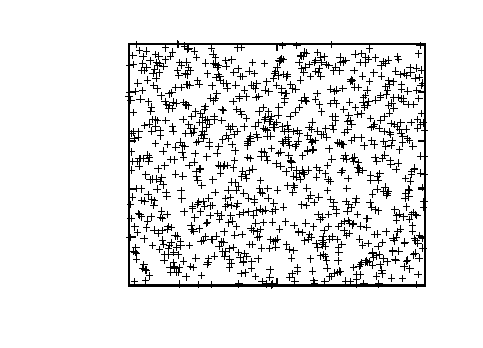
\includegraphics{synapses_before}}%
\put(4500,0){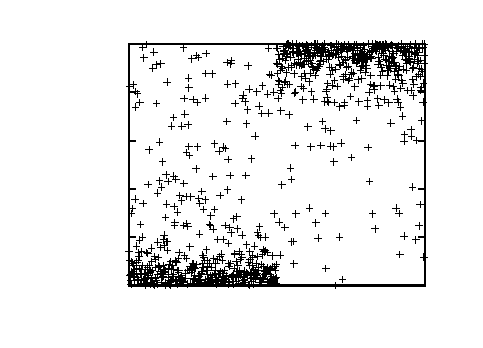
\includegraphics{synapses_after}}%
    \gplfronttext
  \end{picture}%
\endgroup

\end{center}
\caption{Synapse strengths before and after in Song and Abbotts simple model. At first they are all random, after the STDP has had an effect the synapses from one of the two groups have approached their maximum value, the others are near zero. \label{fig:before_after}}
\end{figure}

\begin{thebibliography}{10}

\bibitem{AbbottEtAl1997a}
Abbott LF, Varela JA, Sen K and Nelson SB. (1997) Synaptic depression and cortical gain control. 
\newblock Science, 275: 221--224.

\bibitem{Hebb1949a}
Hebb DO. (1949) The Organization of Behavior. 
\newblock New York: Wiley \& Sons.

\bibitem{MarkramSakmann1995a}
Markram H, Sakmann B (1995) Action potentials propogating back into dendrites triggers changes in efficacy of single-axon synapses between layer V pyramidal cells. 
\newblock Society of Neuroscience Abstract 21.

\bibitem{MarkramEtAl1997a}
Markram H, {L\"{u}bke} J, Frotscher M, Sakmann B (1997) Regulation of synaptic
  efficacy by coincidence of postsynaptic aps and epsps.
\newblock Science 275: 213-215.

\bibitem{BellEtAl1997a} 
Bell CC, Han VZ, Sugawara Y, Grant K (1997) Synaptic plasticity in a
cerebellum-like structure depends on temporal order.
\newblock Nature 387: 278--281.

\bibitem{MageeJohnston1997a}
Magee JC, Johnston D (1997) A synaptically controlled, associative signal for
  Hebbian plasticity in hippocampal neurons.
\newblock Science 275: 209--213.

\bibitem{DebanneGahwilerThompson1998a}
Debanne D, {G\"{a}hwiler} BH, Thompson SM (1998) Long-term synaptic plasticity
  between pairs of individual ca3 pyramidal cells in rat hippocampal slice
  cultures.
\newblock Journal of Physiology 507: 237--247.

\bibitem{ZhangTaoHoltHarrisPoo1998a}
Zhang LI, Tao HW, Holt CE, Harris WA, Poo MM (1998). A critical window for cooperation and competition among developing retinotectal synapses. 
\newblock Nature 395: 37--44.

\bibitem{BiPoo1998a}
Bi G, Poo M (1998) Synaptic modifications in cultured hippocampal neurons:
  Dependence on spike timing, synaptic strength, and postsynaptic cell type.
\newblock Journal of Neuroscience 18: 10464--10472.

\bibitem{SongEtAl2000a}
Song S, Miller K, Abbott L (2000) Competitive hebbian learning through
  spike-timing-dependent synaptic plasticity.
\newblock Nature Neuroscience 3: 919--926.

\bibitem{SongAbbott2001a}
Song S, Abbott L (2001) Cortical development and remapping through spike
  timing-dependent plasticity.
\newblock Neuron 32: 339-350.


\end{thebibliography}

\end{document}
